%This file contains the tex code of my project report for my Data Structure course.
%Author: 章凌豪 / Zhang Linghao <zlhdnc1994@gmail.com>

\section{算法分析}

\subsection{数据结构}

本课程设计中选用的数据结构为Dynamic Tree Bitmap。这是一种基于多分支Trie的动态数据结构。\\
\indent
每个DTBM结点代表了一棵高度为$S - 1$的满二叉树。而这棵满二叉树又相当于一棵有$2^{S}-1$个结点的Binary Trie。与Binary Trie为每个结点开辟空间并用一个位标记来表示是否存在结束于当前结点的前缀不同,我们将一个DTBM结点所代表的树中的结点按层次遍历的顺序组成一个$Internal Bitmap$,它的哪一位为$1$就说明存在一条对应的前缀。\\
\indent
此外,每个DTBM结点还有一个$External Bitmap$,用于表示在多分支Trie意义下该结点的哪些位置挂着子结点。\\
\indent
图3是DTBM的一个例子:\\

\begin{figure}[h!]
\centering
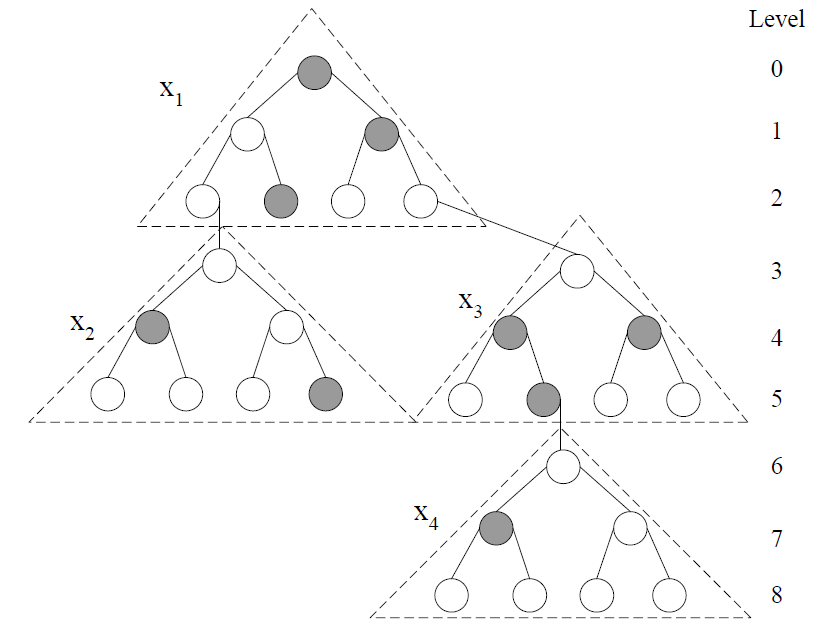
\includegraphics[scale=0.6]{dtbm_eg.png}
\caption{图3}
\end{figure}

\indent
在实际实现时,每个DTBM结点有以下域:
\begin{itemize}
\item $IBM$:用于记录$Internal Bitmap$。在DTBM的实现中,IBM是一个整型,它在二进制表示下的每一位标记了对应前缀的存在与否。
\item $EBM$:用于记录$External Bitmap$。在DTBM的实现中,$EBM$由$2^{S}$个指向子结点的指针组成。
\item $count$:用于记录该结点有多少个$EMB$指针。
\item $nextHop$:用于记录该结点中存在的前缀所对应的下一跳端口。
\end{itemize}

\indent
图4是对应图3中的DTBM的结构。\\

\begin{figure}[h!]
\centering
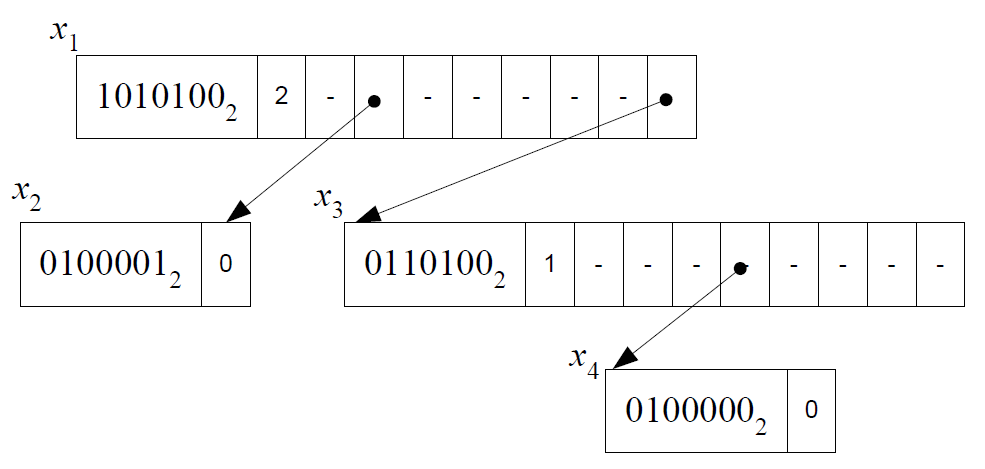
\includegraphics[scale=0.6]{dtbm_struct.png}
\caption{图4}
\end{figure}

\subsection{查找操作}

查找一个IP地址$P$时,我们从根结点出发,每次计算$P.bits(S)$在当前节点中的匹配长度$matchLength$,并检查$IBM$中对应的位是否为1。其中$P.bits(S)$表示当前$P$的前$S$位。\\
\indent
若为1,则说明当前结点中存在一个与待查找的IP地址匹配的前缀。用$bestMatch$和$hopIndex$记录下当前节点以及匹配的前缀所对应的下一跳端口在$nextHop$中的下标。\\
\indent
这一步完成后,我们通过指针$EBM[P.bits(S)]$移动到对应于$P.bits(S)$的子结点,并将$P$左移$S$位。\\
\indent
如此反复,直到走到一个空结点为止。\\
\indent
此时$bestMatch$中储存的即为最后也是最长的一个与待查的IP地址匹配的前缀所在的结点。利用$hopIndex$即可获取查询结果。\\
\indent
其中$matchLength$的求法如下:\\
\indent
对于给定的$P.bits(S)$,它所对应的结点$i$在树中的位置是$2^{H} + P.bits(H)$。其中$H$是树的高度,显然$H = S - 1$。\\
\indent
如果树中存在某一长度的与$P$匹配的前缀,那一定在$i$到根的路径上。利用完全二叉树的性质,$i$的父结点的下标可以简单地由$i/2$得到。\\
\indent
算法如下:

\begin{algorithm}
\NoCaptionOfAlgo
\caption{$Lookup(P)$}
	\Begin{
		$currentNode \leftarrow root$\;
		\Repeat{$currentNode = null$}{
			$matchLength \leftarrow currentNode.IBM.Match(P)$\;
			\If{$matchLength \geq 0$}{
				$bestMatch \leftarrow currentNode$\;
				$hopIndex \leftarrow 2^{matchLength} + P.bits(matchLength)$\;
			}
			$currentNode \leftarrow currentNode.EBM[P.bits(S)]$\;
			Shift $P$ by $S$ bits\;
		}
		\KwRet{$bestMatch.nextHop[hopIndex]$}
	}
\end{algorithm}

\begin{algorithm}
\NoCaptionOfAlgo
\caption{$Match(P)$}
	\Begin{
		$i \leftarrow 2^{H} + P.bits(H)$\;
		$length \leftarrow H$\;
		\While{$i > 0 \kwAnd IBM(i) = 0$}{
			$i \leftarrow i / 2$\;
			$length \leftarrow length - 1$\;
		}
		\KwRet{$length$}\;
	}
\end{algorithm}

\subsection{插入操作}

插入一个前缀$P$时,我们先一边左移$P$一边往下走,直到$P$的长度不足$S$或是当前节点不存在对应$P.bits(S)$的$EBM$指针为止。\\
\indent
如果是后面一种情况,我们就要创建新的结点,直到$P$的长度不足$S$为止。这时要注意设置对应的$EBM$指针并更新$EBM$指针的计数。\\
\indent
然后就可以将$P$插入到当前结点。类似地,$P.bits(P.length)$在$IBM$中对应的下标为$i = 2^{P.length} + P.bits(P.length)$。\\
\indent
算法如下:

\begin{algorithm}
\NoCaptionOfAlgo
\caption{$Insert(P)$}
	\Begin{
		\If{$root = null$}{
			$root \leftarrow \kwNew Node$\;
		}
		\While{$P.length \geq S \kwAnd currentNode.EMB[P.bits[S]] \neq null $}{
			$currentNode \leftarrow currentNode.EBM[P.bits[S]]$\;
			Shift $P$ by $S$ bits\;
		}
		\If{$P.length \geq S$}{
			$currentNode.count \leftarrow currentNode.count + 1$\;
			\Repeat{$P.length < S$}{
				$currentNode.EBM[P.bits[S]] \leftarrow \kwNew Node$\;
				$currentNode \leftarrow currentNode.EBM[P.bits[S]]$\;
				$currentNode.count \leftarrow 1$\;
				Shift $P$ by $S$ bits\;
			}
		}
		Insert $P$ into $currentNode$\;
	}
\end{algorithm}

\subsection{删除操作}

删除一个前缀$P$时,可能出现由于$P$的删除导致一条链上的结点都成为空结点而需要删除的情况。\\
\indent
所以我们在往下走时要将所有$count = 1$且$IBM = 0$的结点都记录下来,因为当这一条链的末尾被删除后,这些结点既不记录前缀,也没有了$EBM$指针,就成为了空结点。\\
\indent
注意在往下走时只要遇到一个不满足上述条件的结点,最后就不需要删除整条链。我们用$nonWeakNode$记录这个结点。\\
\indent
除此之外删除操作与插入操作大致相同,算法如下:

\begin{algorithm}
\NoCaptionOfAlgo
\caption{$Delete(P)$}
	\Begin{
		$currentNode \leftarrow root$\;
		$nonWeakNode \leftarrow null$\;
		\While{$P.length \geq S \kwAnd currentNode \neq null$}{
			\If{$currentNode.count = 1 \kwAnd currentNode.IBM = 0$}{
				Push $currentNode$ and $P.bits[S]$ into stack\;
			}
			\Else{
				Empty the stack\;
				$nonWeakNode \leftarrow currentNode$\;
			}
			$currentNode \leftarrow currentNode.EBM[P.bits[S]]$\;
			Shift $P$ by $S$ bits\;
		}
		\If{$currentNode \neq null \kwAnd P \kwIn currentNode$}{
			Delete $P$ from $currentNode$\;
			\If{$currentNode.count = 0 \kwAnd currentNode.IBM = 0$}{
				Delete empty nodes and set corresponding EBM pointers to $null$\;
			}
		}
	}
\end{algorithm}
	
\subsection{时空复杂度分析}

从理论上讲,选用步长$S$可以将树的高度压缩到$\lceil\frac{W}{S}\rceil$,从而使得各项操作最多只要访问$O(\lceil\frac{W}{S}\rceil)$个结点即可完成。在此基础上还有一些其他因素影响到不同操作的耗时:
\begin{itemize}
\item 对于查询操作来说,在每个结点内需要计算$matchLength$,每次最多要进行$H$次位比较,对耗时影响不大。
\item 对于插入和删除操作来说,由于需要申请和释放内存空间,涉及到如何管理内存的问题,将在3.3节中讨论。但由于数据规模并不大,所以简单地使用\textbf{malloc()}和\textbf{free()}来管理内存也不会成为性能的瓶颈。
\end{itemize}
总的来说,各项操作的复杂度基本相同。在实现中由于选用$S = 5$,所以树的高度被压缩到了$7$,虽然与朴素的Binary Tree相比,DTBM的各项操作在常数上会大一些,但整体性能还是十分优秀的。\\
\indent
由于DTBM动态维护结点,所以很难精确地计算空间消耗,但根据DTBM结点的结构可以知道空间复杂度大致是$O(2^{S}N')$的,其中$N'$是结点数。一般情况下$N' < N$,且根据路由前缀的密集程度不同,$N'$有可能会很小。极端情况下,对于每个前缀我们都要创建一条到树底的链,所以$N'$的上限是$\lceil\frac{W}{S}\rceil N$,在实际中这个上限是完全不可能达到的。\\
\indent
经过实际数据测试后发现,DTBM的空间消耗是完全可以接受的。\\
\indent
当将算法拓展到IPv6地址时,我们会发现除了$W$从$32$变为$128$以外,其他的一切都不需要变动。假设我们继续使用$S = 5$,树的高度就是$26$,变为原来的$4$倍左右,所以各项操作的常数会乘上一个$4$,仅此而已。\\
\indent
类似地,空间消耗也会随之增加。此时在比较坏的情况下,空间的确有可能会成为一个瓶颈,但现实情况是当前IPv6路由表项数目还非常少。当有一天IPv6路由表项数目逼近现在的IPv4路由表项数目时,新的算法自然会应运而生。\\

\clearpage
